\documentclass{article} % For LaTeX2e
\usepackage{nips14submit_e,times}
\usepackage{hyperref}
\usepackage{url}

\usepackage{amsmath,bm}
\usepackage{amssymb}
\usepackage{algorithm}
\usepackage{algorithmic}
\usepackage{graphicx}
\usepackage{tabularx}
\usepackage{array,arydshln}
\usepackage{subcaption}
%\documentstyle[nips14submit_09,times,art10]{article} % For LaTeX 2.09

\title{A Multimodal Recurrent Neural Networks for Generating Novel Sentence Level Image Descriptions}


\author{
Junhua Mao\\
Host: Wei Xu\\
Yi Yang and Jiang Wang
}

% The \author macro works with any number of authors. There are two commands
% used to separate the names and addresses of multiple authors: \And and \AND.
%
% Using \And between authors leaves it to \LaTeX{} to determine where to break
% the lines. Using \AND forces a linebreak at that point. So, if \LaTeX{}
% puts 3 of 4 authors names on the first line, and the last on the second
% line, try using \AND instead of \And before the third author name.

\newcommand{\fix}{\marginpar{FIX}}
\newcommand{\new}{\marginpar{NEW}}

% \nipsfinalcopy % Uncomment for camera-ready version

\begin{document}

\maketitle

% To do:
% The two application paragraph. Waiting for the results.
\vspace{-1em}
\begin{abstract}

In this paper, we present a multimodal Recurrent Neural Network (m-RNN) model for generating novel sentence descriptions to explain the content of images.
It directly models the probability distribution of generating a word given previous words and the image.
Image descriptions are generated by sampling from this distribution.
The model consists of two sub-networks: a deep recurrent neural network for sentences and a deep convolutional network for images. 
These two sub-networks interact with each other in a multimodal layer to form the whole m-RNN model.
% three multimodal tasks: sentence generation, sentence retrieval given query image, and image retrieval given query sentence.
% Unlike some previous methods that map both the image and sentence features into a common semantic space, we directly model the probability distribution of generating a word given previous words.
% The image descriptions can be generated by sampling from the word probability distribution.
% It serves as the affinity metric between image and sentence for the retrieval tasks. 
The effectiveness of our model is validated on three benchmark datasets (IAPR TC-12 \cite{grubinger2006iapr}, Flickr 8K \cite{rashtchian2010collecting}, and Flickr 30K \cite{hodoshimage}).
Our model outperforms the state-of-the-art generative method.
In addition, the m-RNN model can be applied to retrieval tasks for retrieving images or sentences, and achieves significant performance improvement over the state-of-the-art methods which directly optimize the ranking objective function for retrieval.

\end{abstract}
% To do:

\section{Introduction}

Obtaining sentence level descriptions for images is becoming an important task and has many applications, such as early childhood education, image retrieval, and navigation for the blind.
Thanks to the rapid development of computer vision and natural language processing technologies, recent works have made significant progress for this task (see a brief review in Section \ref{sec:related_work}).
Many of these works treat it as a retrieval task.
They extract features for both sentences and images, and map them to the same semantic embedding space.
These methods address the tasks of retrieving the sentences given the query image or retrieving the images given the query sentences.
But they can only label the query image with the sentence annotations of the images already existing in the datasets, thus lack the ability to describe new images that contain previously unseen combinations of objects and scenes.

In this work, we propose a multimodal Recurrent Neural Networks (m-RNN) model to address both the task of generating novel sentences descriptions for images, and the task of image and sentence retrieval.
The whole m-RNN architecture contains a language model part, an image part and a multimodal part.
The language model part learns the dense feature embedding for each word in the dictionary and stores the semantic temporal context in recurrent layers.
The image part contains a deep Convulutional Neural Network (CNN) \cite{krizhevsky2012imagenet} which extracts image features.
The multimodal part connects the language model and the deep CNN together by a one-layer representation.
Our m-RNN model is learned using a perplexity based cost function (see details in Section \ref{sec:trainCost}).
The errors are backpropagated to the three parts of the m-RNN model to update the model parameters simultaneously.
To the best of our knowledge, this is the first work that incorporates the Recurrent Neural Network in a deep multimodal architecture.

In the experiments, we validate our model on three benchmark datasets: IAPR TC-12 \cite{grubinger2006iapr}, Flickr 8K \cite{rashtchian2010collecting}, and Flickr 30K \cite{hodoshimage}.
we show that our method significantly outperforms the state-of-the-art methods in both the task of generating sentences and the task of image and sentence retrieval when using the same image feature extraction networks.
% Some examples are shown in Figure \ref{fig:res_example}.
Our model is extendable and has the potential to be further improved by incorporating more powerful deep networks for the image and the sentence.
% To do:
% aaai12's paper (not important)

\begin{figure}[tb!]
\begin{center}
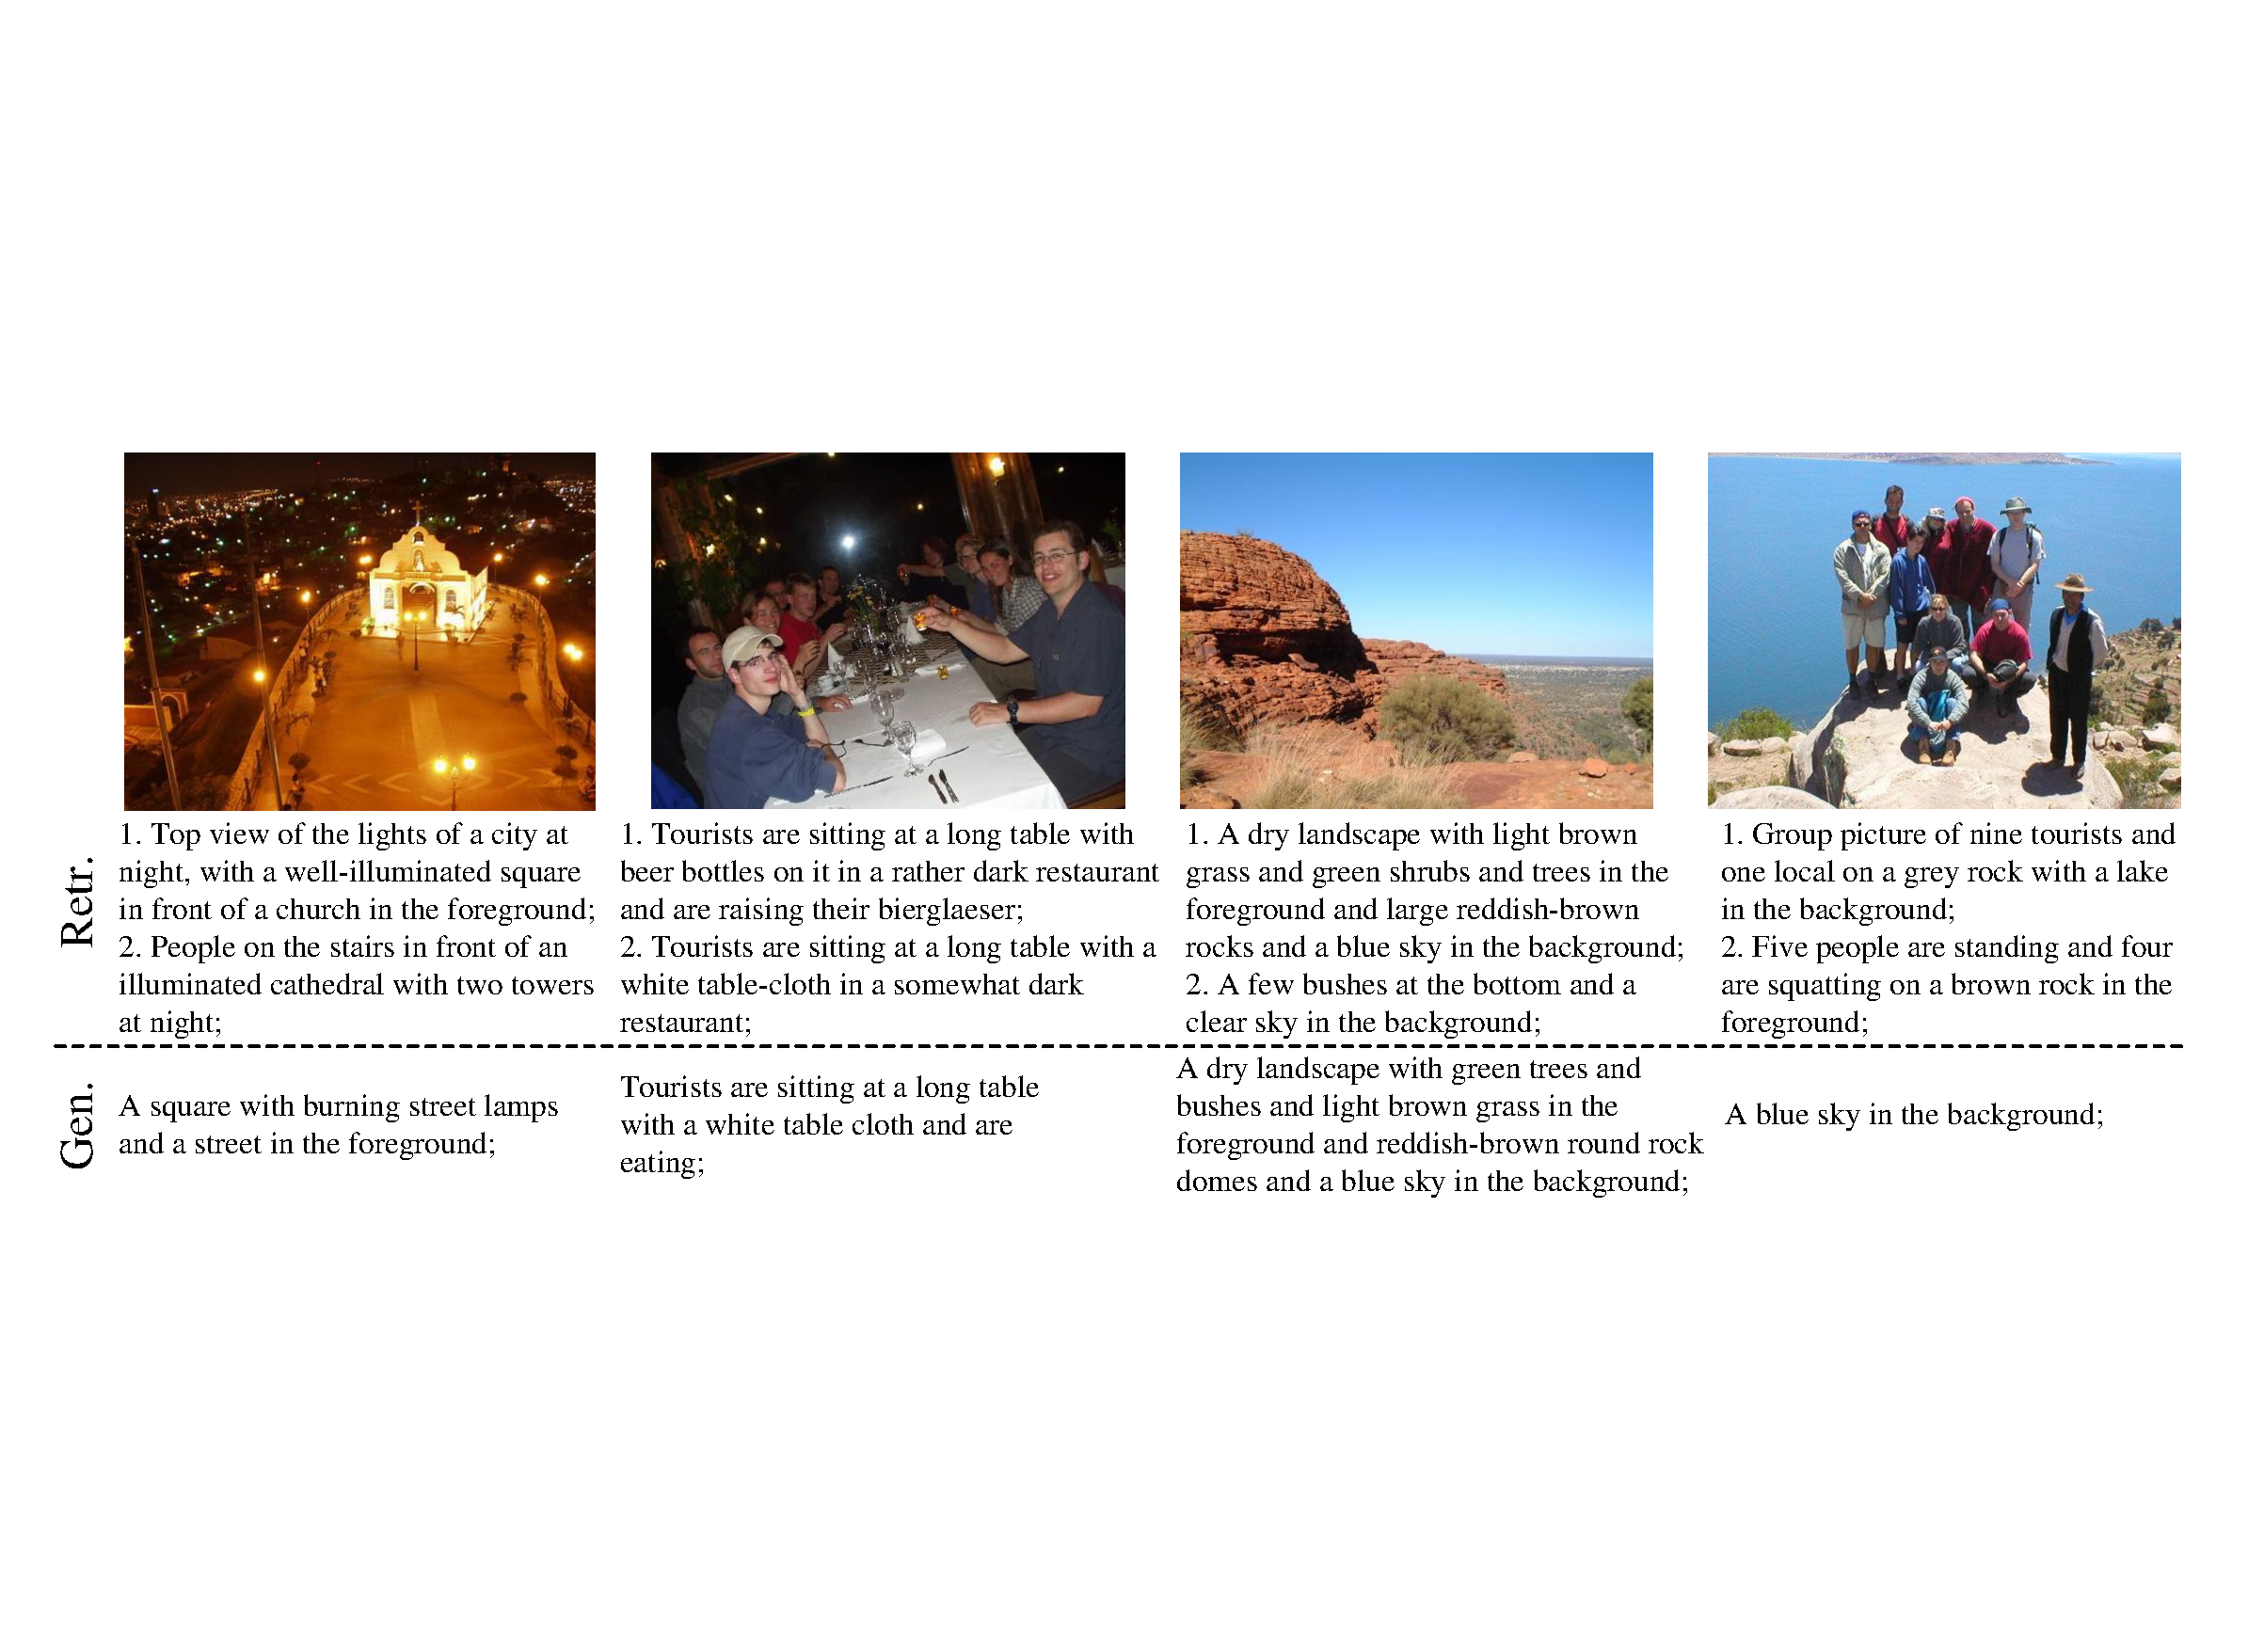
\includegraphics[width=0.98\linewidth]{PaperFigures/res_example.pdf}
\end{center}
   \caption{Examples of the generated and two top-ranked retrieved sentences given the query image from IAPR TC-12 dataset.
   The sentences can well describe the content of the images.
   We show a failure case in the fourth image, where the model mistakenly treats the lake as the sky.
   }
\label{fig:res_example}
\end{figure}

\section{Related Work}
\label{sec:related_work}

\textbf{Deep model for computer vision and natural language.}
The deep neural network structure develops rapidly in recent years in both the field of computer vision and natural language.
For computer vision, Krizhevsky et. al \cite{krizhevsky2012imagenet} proposed a deep convolutional neural networks with 8 layers (denoted as AlexNet) for image classification tasks and outperformed previous methods by a large margin.
Recently, Girshick et. al \cite{girshick2014rcnn} proposed a object detection framework based on AlexNet.
For natural language, the Recurrent Neural Network shows the state-of-the-art performance in many tasks, such as speech recognition and word embedding learning \cite{mikolov2010recurrent,mikolov2011extensions,mikolov2013distributed}.

\textbf{Image-sentence retrieval.}
Many works treat the task of describe images as a retrieval task and formulate the problem as a ranking or embedding learning problem \cite{hodosh2013framing,frome2013devise,socher2014grounded}.
They will first extract the word and sentence features (e.g. Socher et.al \cite{socher2014grounded} uses dependency tree Recursive Neural network to extract sentence features) as well as the image features.
Then they optimize a ranking cost to learn an embedding model that maps both the language feature and the image feature to a common semantic feature space.
In this way, they can directly calculate the distance between images and sentences.
Most recently, Karpathy et.al \cite{karpathy2014fragment} showed that object level image features based on object detection results will generate better results than image features extracted at the global level.

\textbf{Generating novel sentence descriptions for images.}
There are generally two categories of methods for this task.
The first category assumes a specific rule of the language grammar.
They parse the sentence and divide it into several parts \cite{mitchell2012midge,gupta2012image}.
Then each part is associated to a object or an attribute in the image (e.g. \cite{kulkarni2011baby} uses a Conditional Random Field model and \cite{farhadi2010every} uses a Markov Random Field model).
This kind of method generates sentences that are syntactically correct.
Another category of methods, which is more related to our method, learns a probability density over the space of multimodal inputs (i.e. sentences and images), using for example, Deep Boltzmann Machines \cite{srivastava2012multimodal}, and topic models \cite{barnard2003matching,jia2011learning}.
They can generate sentences with richer and more flexible structure than the first group.
The probability of generating sentences given the corresponding image can serves as the affinity metric for retrieval.
Our method falls into this category.
More close related to our tasks and method is the work of Kiros et al. \cite{kiros2013multimodal}, which is built on a Log-BiLinear model \cite{mnih2007three}.
It needs a fixed length of context (i.e. five words), whereas in our model, the temporal context is stored in a recurrent architecture, which allows arbitrary context length.

% To do:
% Wei: Recurrent layer is concatnateded or added with the previous layers?. (add)
% Do we need to mention the norm?

\section{Model Architecture}

\begin{figure}[htb]
\begin{center}
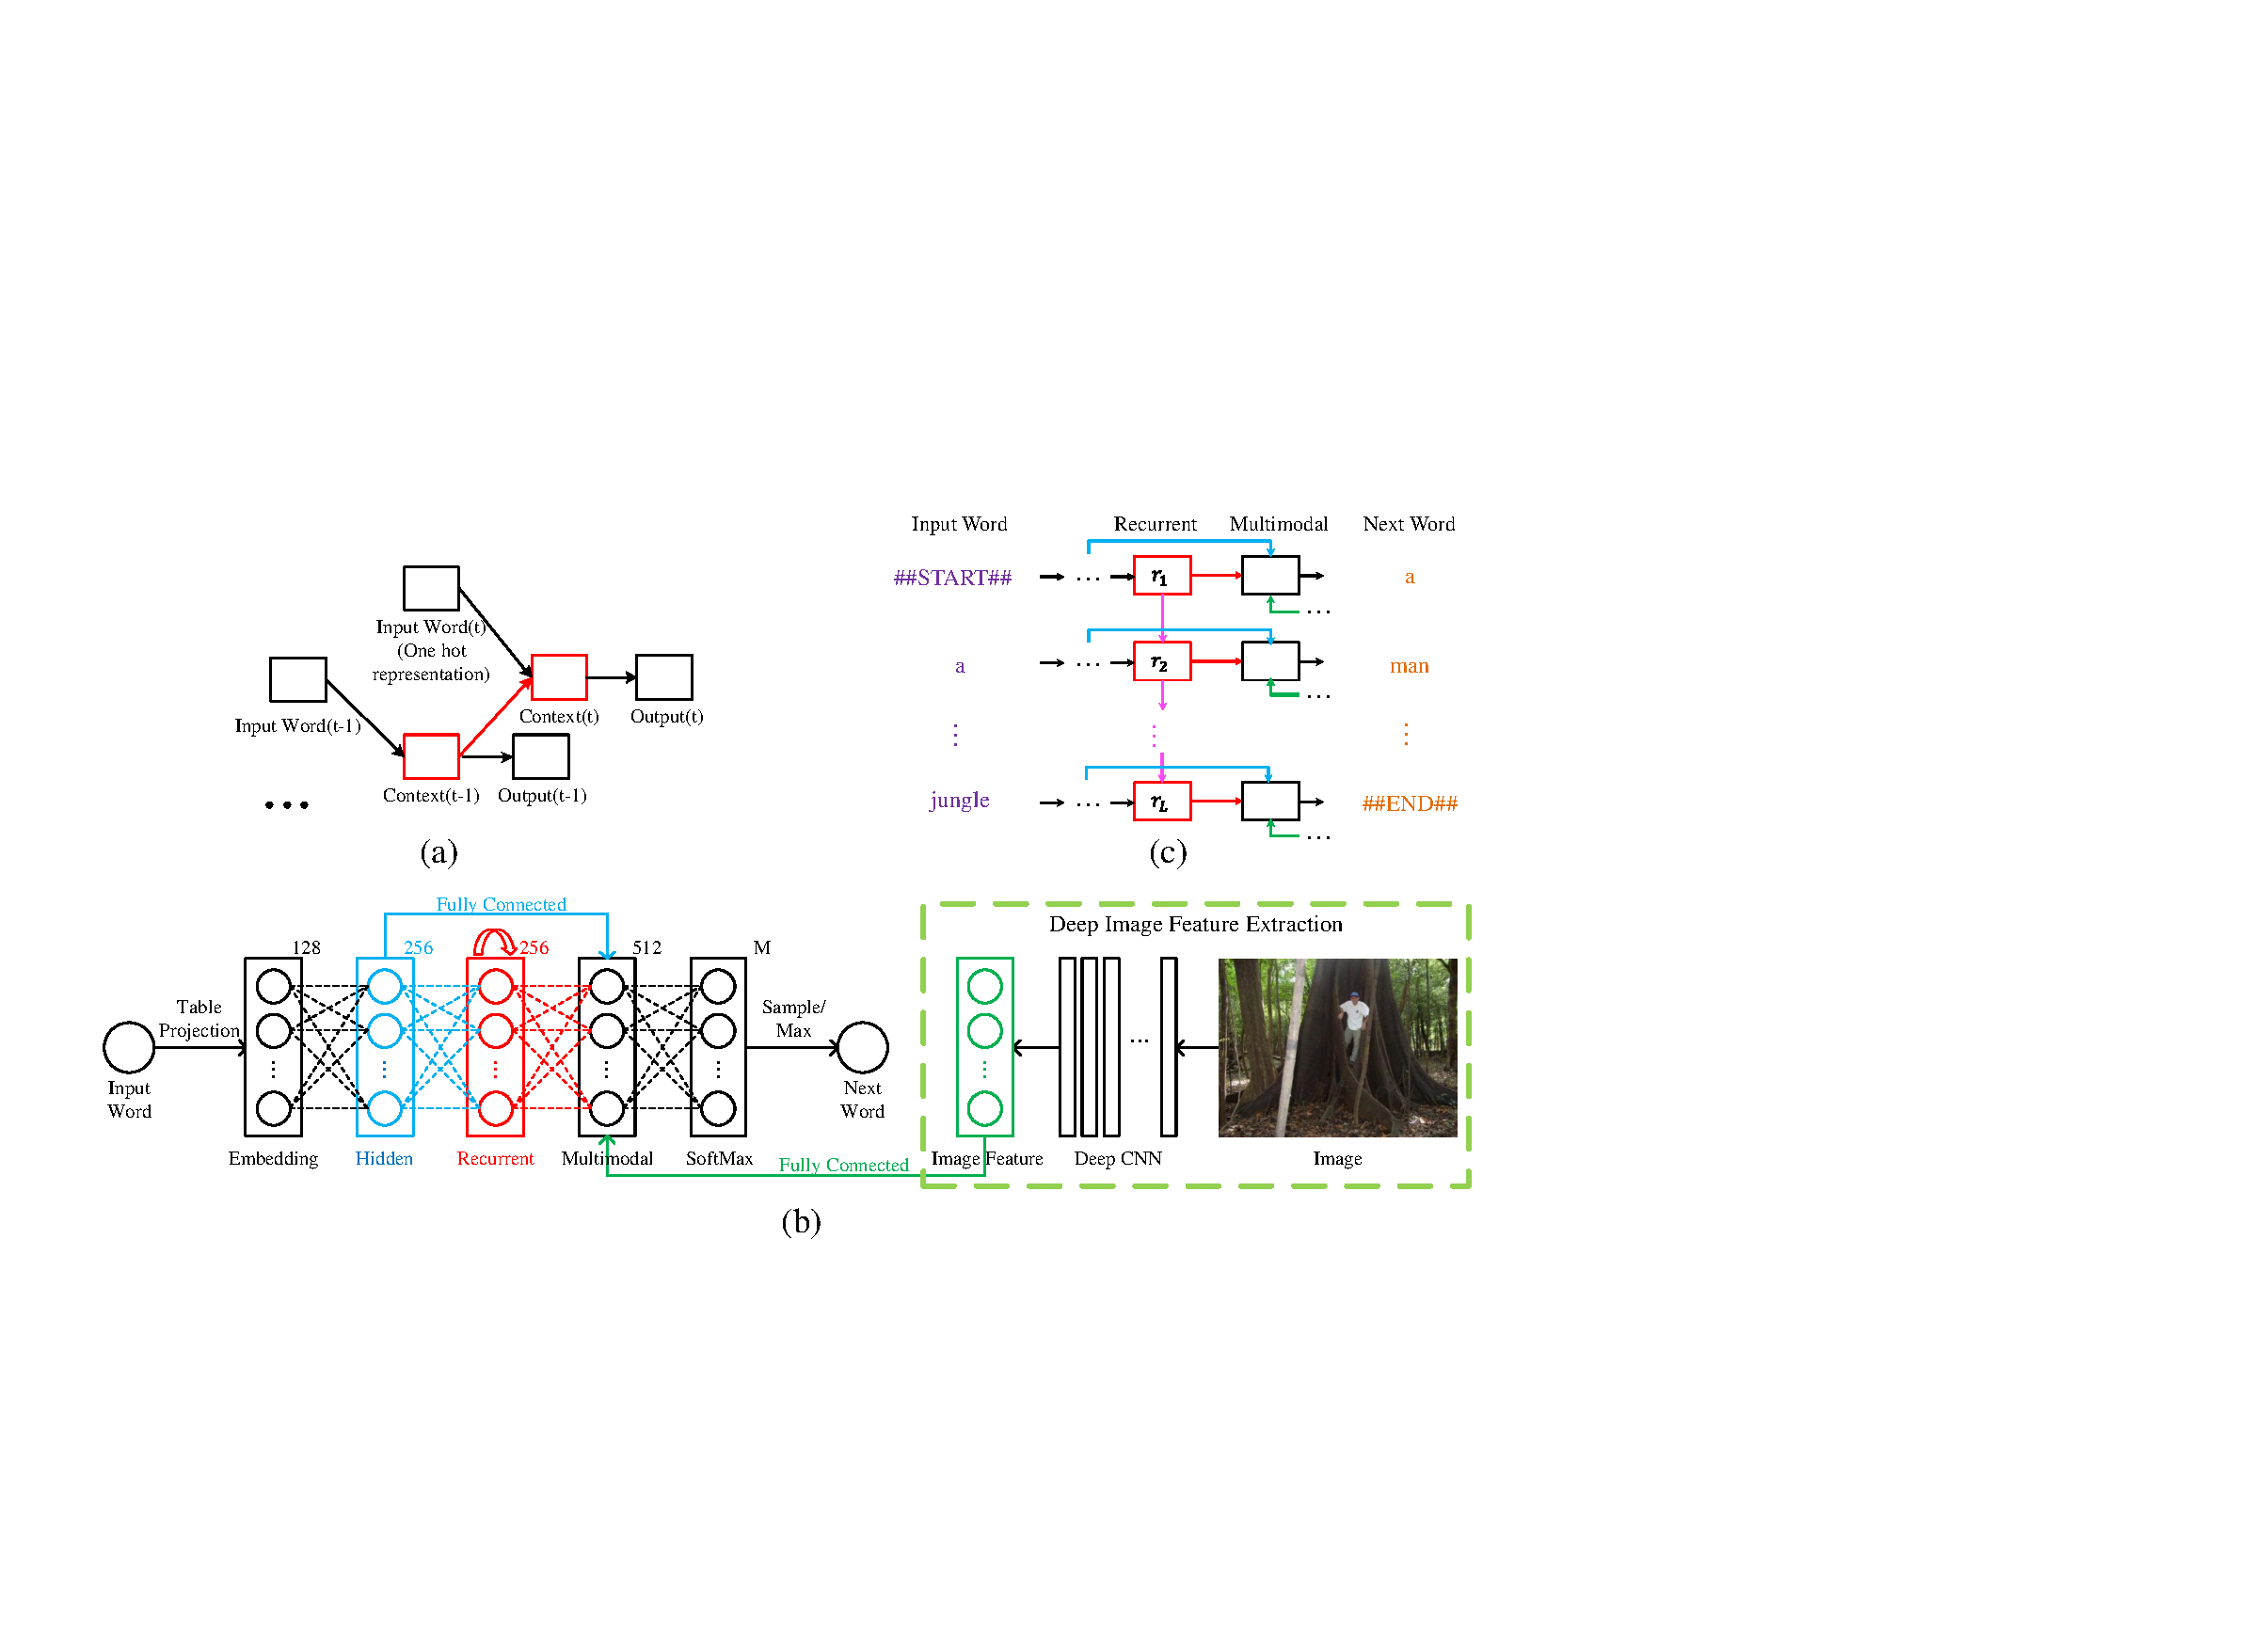
\includegraphics[width=0.95\linewidth]{PaperFigures/arch_final_visio.pdf}
\end{center}
   \caption{Illustration of the basic Recurrent Neural Network (RNN) and our multimodal Recurrent Neural Network (m-RNN) architecture.
   (a). The basic RNN architecture. 
   (b). The architecture of m-RNN model.
   The input of the model is an image and its corresponding sentences. (e.g. the sentence for the shown image is: \emph{a man at a giant tree in the jungle}. 
   The model will estimate the probability distribution of the next word given previous words and the image.
   This architecture is deeper than the basic RNN.
   % of structure without considering the extendibility of the recurrent layer.
   (c). The illustration of how the recurrent layer works in m-RNN. 
   % We can unfold the recurrent layer, which leads to the temporal depth of the network.
   The model parameters are shared for each temporal session of the unfolded m-RNN model.
   }
\label{fig:illu_RNN}
\end{figure}

% For layer \textcircled{\raisebox{-0.9pt}{1}} and layer \textcircled{2},
\subsection{Basic recurrent neural network}
We briefly introduce the basic Recurrent Neural Network (RNN) \cite{elman1990finding,mikolov2010recurrent,mikolov2011extensions} that is widely used for many natural language processing tasks, such as speech recognition.
Its architecture is shown in Figure \ref{fig:illu_RNN}(a).
It has three types of layers in each time session: the input word layer $\mathbf{w}$, the context layer $\mathbf{s}$ and the output layer $\mathbf{y}$.
The activation of input, context and output layers in time $t$ is denoted as $\mathbf{w}(t)$, $\mathbf{s}(t)$, and $\mathbf{y}(t)$.
$\mathbf{w}(t)$ is the one-hot representation of the current word. 
This representation is binary, and has the same dimension of the vocabulary size with only one non-zero element.
$y(t)$ can be calculated as follows:
\begin{equation}
\mathbf{x}(t) = [\mathbf{w}(t)^T\ \ \mathbf{s}(t-1)^T]^T;\ \ \ 
\mathbf{s}(t)=f_1(\mathbf{U} \cdot \mathbf{x}(t));\ \ \ 
\mathbf{y}(t)=g_1(\mathbf{V} \cdot \mathbf{s}(t));
\end{equation}
where $\mathbf{x}(t)$ as a vector that concatenates $\mathbf{w}(t)$ and $\mathbf{s}(t-1)$, $f_1(.)$ and $g_1(.)$ are element-wised sigmoid and softmax function respectively.

We define two types of ``depths'' for a RNN architecture. 
We denote the number of layers in each time session as the \emph{structure depth} (e.g. the structure depth of the basic RNN is 3).
When we compare the depth of different RNN networks, we refer to the structure depth.
The second depth is denoted as the \emph{temporal depth}. 
% Although the structure of the basic RNN model is simple, it is a very deep network which can be unfolded in time sequences.
Accordingly, when we do the backpropagation, we need to propagate the error through recurrent connections back in time \cite{rumelhart1988learning}.

\subsection{Our m-RNN model}
The structure of our multimodal Recurrent Neural Network (m-RNN) is shown in Figure \ref{fig:illu_RNN}(b).
The m-RNN model is much deeper than the basic RNN model.
Its structure depth is 7 (i.e. input word layer, word embedding layer, hidden layer, recurrent layer, multimodal layer, softmax layer and the next word layer).

The word embedding layer learns a initial dense word embedding representation to replace the one-hot representation in basic RNN.
It has several advantages.
Firstly, it will significantly lower the number of parameters in the networks because the dense word vector (128 dimension) is much smaller than the one-hot word vector.
Secondly, the dense word embedding encodes the semantic meanings of the words.
We can find the semantically relevant words by calculating the Euclidean distance between two dense word vectors.

Most of the sentence-image multimodal models \cite{karpathy2014fragment,frome2013devise,socher2014grounded,kiros2013multimodal} use pre-computed word embedding vectors as the initialization of their model. 
In contrast, we randomly initialize our word embedding layers and learn them from the training data.
We show that this random initialization is enough for our architecture to generate the state-of-the-art results.
To further refine the word representation, we add a hidden layer after the initial word embedding layer and treat the activation of the hidden layer as the final word representation.

After the hidden layer, we have a recurrent layer with 256 dimensions.
The calculation of the recurrent layer is slightly different from the basic RNN.
Instead of concatenating the word representation in time $t$ and the recurrent layer vector in time $t-1$, we first map the word representation in time $t$ and context in time $t-1$ into a same vector space and add them together:
\begin{equation}
\mathbf{s}(t)=f_2(\mathbf{U}_w \cdot \mathbf{w}(t) + \mathbf{U}_s \cdot \mathbf{s}(t-1));
\end{equation}
where $\mathbf{s}$ and $\mathbf{w}$ denotes the recurrent layer vector and the word representation respectively.
% This strategy will reduce the number of parameters and accelerate the training and testing process.

Inspired by the recent success of the Rectified Linear Unit (ReLU) in training very deep structure in computer vision field \cite{krizhevsky2012imagenet}, we replace the element-wised sigmoid function in basic RNN with ReLU function.
ReLU is faster, and harder to saturate or overfit the data than many non-linear functions, such as sigmoid.
Previous methods \cite{mikolov2010recurrent,mikolov2011extensions} need to conduct backpropagation through time (BPTT) \cite{rumelhart1988learning} for RNN suffers from the vanishing gradient problem because even the simplest the RNN model has a large temporal depth.
They need to use some heuristics, such as truncated BPTT, to avoid this problem.
Truncated BPTT will stop the BPTT after $k$ time steps, where $k$ is a hand-defined hyperparameter.
Because of the good properties of ReLU, we do not need to stop the BPTT at early stage, which leads to a better and more efficient utilization of the data than truncated BPTT.

After the recurrent layer, we set up a 512 dimensional multimodal layer that connect the language model part and the image part of the whole m-RNN model.
The language model part includes the hidden layer (the word representation) and the recurrent layer (the language context).
The image part contains the image features.
Here we connect the seventh layer of AlexNet \cite{krizhevsky2012imagenet} to the multimodal layer (please refer to Section \ref{sec:ImgSenFeat} for more details).
But our framework can utilize any image features.
We map the feature vector for each layer to a same feature space and add them together to obtain the feature vector for the multimodal layer:
\begin{equation}
\mathbf{m}(t)=g_2(\mathbf{V}_w \cdot \mathbf{w}(t) + \mathbf{V}_s \cdot \mathbf{s}(t) + \mathbf{V}_I \cdot \mathbf{I});
\end{equation}
where $\mathbf{w}$ denotes the multimodal layer feature vector, $\mathbf{I}$ denotes the image feature, $g_2(.)$ is the element-wised scaled hyperbolic tangent function:
\begin{equation}
g_2(x) = 1.7159 \cdot \tanh( \frac{2}{3} x)
\end{equation}
This function will force the gradients into the most non-linear value range and can accelerate the training process than the basic hyperbolic tangent function \cite{lecun2012efficient}.

%We do not restrict the norm the three feature layers that connect to the multimodal layer.
%Our experiments shows that the L2 norm of the hidden layer, 

As the basic RNN, our m-RNN model has a softmax layer that will generate the probability distribution of next word.
The dimension of this layer is the vocabulary size $M$, which is different for different datasets.

\section{Training Objective}
\label{sec:trainCost}
We use the average logarithm of the \emph{Perplexity} of the sentences in the training set given their corresponding images as the cost function of our m-RNN model.
Perplexity is a standard approach to evaluating language model.
The perplexity for one word sequence (i.e. a sentences) $w_{1:L}$ can be calculated as follows, $L$ is the length of the word sequences:
\begin{equation}
\log_2 \mathcal{PPL}(w_{1:L}|\mathbf{I}) = -\frac{1}{L} \sum_{n=1}^{L} \log_2 P(w_n|w_{1:n-1},\mathbf{I})
\end{equation}
where $\mathcal{PPL}(w_{1:L}|\mathbf{I})$ denotes the perplexity of the sentence $w_{1:L}$ given the image $\mathbf{I}$.
$P(w_n|w_{1:n-1},\mathbf{I})$ is the probability of the current word $w_n$ given $\mathbf{I}$ and previous words $w_{1:n-1}$.
It corresponds to the feature vector of the SoftMax layer of our modal.

The cost function of our model is the average of the logarithm of the perplexity for all the sentences in the training set:
\begin{equation}
\mathcal{C} = -\frac{1}{N} \sum_{i=1}^{N} \log_2 \mathcal{PPL}(w_{1:L}^{(i)}|\mathbf{I}^{(i)})
\end{equation}
where $N$ is the number of sentences in the training set.
It is equivalent to the reciprocal of the geometric mean of the probability for the model to generate the training sentences.
Our training objective is to minimize this cost function, which is equivalent to maximize the probability of the model to generate the sentences in the training set given their corresponding images.
The cost function is derivable thus we can use backpropagation to learn the model parameters.

\section{Learning of Image and Sentence Features}
\label{sec:ImgSenFeat}

The architecture of our model allows the gradients from the loss function to be backpropagated to both the language modeling part (i.e. the word embedding, hidden and the recurrent layers) as well as the image part (e.g. the AlexNet \cite{krizhevsky2012imagenet}).

For the language modeling part, as mentioned above, we randomly initialize the language modeling layers and learn their parameters. For the image part, we connect the seventh layer of a pre-trained Convolutional Neural Network \cite{krizhevsky2012imagenet,donahue2013decaf} (aso denoted as AlexNet).
The same features extract from the seventh layer of AlexNet (also denoted as decaf features \cite{donahue2013decaf}) was widely used by previous multimodal methods \cite{kiros2013multimodal,frome2013devise,karpathy2014fragment,socher2014grounded}.
In a most recent work \cite{karpathy2014fragment}, the same image features combined with the state-of-the-art detection framework of Region-CNN \cite{girshick2014rcnn} were used.
Their experiments showed that using this detection framework will indeed increase the performance.
In the experiments, we will show that our method performs much better than \cite{karpathy2014fragment} when the same image features are used, and even better than their results of more sophisticated detection features in terms of many evaluation metrics.

We can update the AlexNet according to the gradient backpropagated from the multimodal layer. In this paper, we fix the image features and the deep CNN network in the training stage due to the luck of the data (The datasets we used in the experiment have less than 30K images).
In the future work, we will try our method on large dataset and finetune the parameters of the deep CNN network in the training stage.

\section{Sentence Generation, Image and Sentence Retrieval}
After training of the m-RNN model, we can use the model for the tasks of sentence generation, image retrieval using sentences and sentence retrieval using images.

The sentence generation process is straight forward.
Start from the start sign ``\#\#START\#\#'' or any length of the context words (e.g. we can give the first words in the reference sentences), our model can calculate the probability distribution of the next word: $P(w|w_{1:n-1},\mathbf{I})$.
Then we can sample from this probability distribution to pick the next word.
In practice, we find that picking the word with the maximum probability will perform slightly better than sampling.
After that, we input the picked word to the model and sample the next word.
This process repeated until we have the end sign ``\#\#END\#\#''.

For the retrieval tasks, we can use our model to calculate the perplexity of generating a sentence given an image.
The perplexity can be treated as an affinity measurement between sentences and images.
For the image retrieval task, we just need to retrieve the images that generate the minimum perplexity with the sentence query. 

The sentence retrieval tasks is trickier because there might be some sentences that has high probability to any image query.
Instead of looking at the perplexity or the probability of the sentences given the query image, we need to use the normalized probability for each sentence: $P(w_{1:L}|\mathbf{I}) / \sum_{\mathbf{I^{'}}} P(w_{1:L}|\mathbf{I^{'}})$ where $\mathbf{I^{'}}$ are images sampled from the training set, $P(w_{1:L}|\mathbf{I}) = \mathcal{PPL}(w_{1:L}|\mathbf{I}) ^ {-L}$.
% To do:
% Perplexity details, Word Error Rate for training (method section).
% The norm of different layers after training and before training
% Our framework is flexible. (abstract?)
% Do we need to say more about the R@5, R@10 for flickr-30K? (experiment)
% Details of the training: (model description? exp? prefer experiments)
%  1. Number of words in the dictionary
%  2. Word error rate
%  3. Training time
% Finetuning the networks? (future works)

\section{Experiments}

\subsection{Datasets}
We test our method on three benchmark datasets with sentence level annotations: IAPR TC-12 \cite{grubinger2006iapr}, flickr 8K \cite{rashtchian2010collecting}, and flickr 30K \cite{hodoshimage}.

Here are some statistics and our experimental settings for the three datasets:

\textbf{IAPR TC-12 Benchmark}  This dataset consists of around 20,000 images taken from locations around the world.
This includes images of different sports and actions, people, animals, cities, landscapes, and so on.
For each image, they provide at least one sentences annotations.
On average, there are about 1.7 sentences annotations for one image.
We adopt the publicly available separation of training and testing set as previous works \cite{GVS10a,kiros2013multimodal}.
There are 17,665 images for training and 1962 images for testing.

\textbf{Flickr8K Benchmark}  This dataset consists of 8,000 images extracted from Flickr.
For each image, they provide five sentences annotations.
The grammar for the annotations of this dataset is simpler than those of the IAPR TC-12 dataset.
We adopt the standard separation of training, validation and testing set which is provided by the dataset.
There are 6,000 images for training, 1,000 images for validation and 1,000 images for testing.

\textbf{Flickr30K Benchmark}  This dataset is a recent extension of Flickr8K.
It consists of 158,915 crowd-sourced captions describing 31,783 images.
So for each image, they also provide five sentences annotations.
The grammar and style for the annotations of this dataset is similar to Flickr8K.
We follow the previous work \cite{karpathy2014fragment} which used 1,000 images for testing.
This dataset, as well as the Flick8K dataset, is mainly used for the image-sentence retrieval tasks and there is not public available results of methods for generating novel sentence descriptions.

\subsection{Experiments settings}

Our model can be used for three tasks: 1) Sentences generation; 2) Sentence retrieval (retrieval top relevant sentences to the given image); 3) Image retrieval (retrieval top relevant images to the given sentence);

\subsubsection{Evaluation metrics for sentence generation}
Following previous works, we use sentence perplexity and BLEU score \cite{papineni2002bleu,lin2004automatic} as the evaluation metrics.
BLEU score was originally designed for automatically machine translation where the task is to give a score to a translated sentences given several references sentences.
We can treat the sentence generation task as the "translation" of the content of image to sentences.
The drawback of using BLEU in our task is that for some images, the reference sentences might not contains all the elements and content in the image and the BLEU score might penalize the arguably correct generated sentences, though it remains as the standard evaluation metric for sentence generation methods for image.
To conduct a fair comparison, we adopt the same sentence generation steps and experiment settings as \cite{kiros2013multimodal}, and generate as many words as there are in the reference sentences.
Note that our model actually do not need to know the length of the reference sentence because we add a end sign "\#\#END\#\#" at the end of every training sentences and we can stop the generation process when our model outputs the word "\#\#END\#\#".

\subsubsection{Evaluation metrics for sentence retrieval and image retrieval}
\label{sec:EvaRet}
For Flickr8K and Flickr30K datasets, we adopted the same evaluation metrics as previous works \cite{socher2014grounded,frome2013devise,karpathy2014fragment} for both the tasks of sentences retrieval and image retrieval.
They used R@K (K = 1, 5, 10), which is the recall rate of the first groundtruth sentences (sentence retrieval task) or images (image retrieval task) as the measurements.
Higher R@K usually means better retrieval performance of different methods.
Since we care most of the top retrieved results, the R@K with smaller K is more important than those with larger K.
In addition to R@K, they used the Med r, which is the median rank of the first groundtruth sentences (sentence retrieval task) or images (image retrieval task).
Lower Med r usually means better performance.

For IAPR TC-12 datasets, we adopt exactly the same evualation metrics as \cite{kiros2013multimodal}, which plotted the mean number of matches of the retrieved groundtruth sentences or images with respect to the percentage of the retrieved sentences or images for the testing set.
For sentences retrieval task, \cite{kiros2013multimodal} used a shortlist of 100 images which are the nearest neighbors of specific testing image in the image feature space.
This shortlist makes the task harder because similar images might have similar descriptions and it is often harder to find the subtle difference among the sentences and pick the most suitable one.
Although there is no published R@K score and Med r score for this dataset as the best of our knowledge, we also report these metrics of our method for future comparison.

\subsection{Results on IAPR TC-12}

\begin{table}[htb]
	\centering
\begin{tabular}{l|cccc}
\hline
      & PERP  & B-1   & B-2   & B-3 \\
\hline
BACK-OFF GT2 & 54.5  & 0.323 & 0.145 & 0.059 \\
BACK-OFF GT3 & 55.6  & 0.312 & 0.131 & 0.059 \\
LBL \cite{mnih2007three}  & 20.1  & 0.327 & 0.144 & 0.068 \\
MLBL-B-DeCAF \cite{kiros2013multimodal} & 24.7  & 0.373 & \textbf{0.187} & 0.098 \\
MLBL-F-DeCAF \cite{kiros2013multimodal} & 21.8  & 0.361 & 0.176 & 0.092 \\
Gupta et al. \cite{gupta2012choosing} & /     & 0.15  & 0.06  & 0.01 \\
Gupta \& Mannem \cite{gupta2012image} & /     & 0.33  & 0.18  & 0.07 \\
\hdashline
Ours-RNN-Base & 7.77  & 0.3134 & 0.1168 & 0.0803 \\
Ours-m-RNN & \textbf{6.92} & \textbf{0.3951} & 0.1828 & \textbf{0.1311} \\
\hline
\end{tabular}%
	\caption{Results of generated sentences in the iaprtc-12 dataset. }
	\label{tab:iaprtc_gen}
\end{table}

The results of generated sentences is shown in Table \ref{tab:iaprtc_gen}.
BACK-OFF GT2 and GT3 are n-grams methods with Katz backoff and Good-Turing discounting \cite{chen2000survey,kiros2013multimodal}.
Ours-RNN-Base has the same architecture with our m-RNN model except that we will not input the image features to the network.
It serves as a baseline for our m-RNN model.

To conduct a fair comparison, we followed the same experimental settings of \cite{kiros2013multimodal}, includes the context length to calculate the BLEU score and perplexity.
Please note that the perplexity is calculated according to the conditional probability of the words given all of its previous reference words in the sentences.
Therefore, a strong language model that successfully captures the grammar of sentences can have a low perplexity without the image content. 
Perplexity does not directly correlate to the BLEU score where we need to sample the words from the probability distribution generated by the model.
For example, although for this dataset, our baseline method of RNN can generate a very low perplexity, it failed to generated sentences with high quality since its BLEU score is not very high.
From this perspective, the BLEU score is a better measurement for the generating sentences.

From the experiments, we can see that our m-RNN model performs much better than our baseline RNN model in terms of both perplexity and BLEU score.
It also outperforms the state-of-the-art methods in terms of perplexity, B-1, B-3, and a comparable result for B-2.

For retrieval tasks, as mentioned in Section \ref{sec:EvaRet}, we draw a recall accuracy curve with respect to the percentage of retrieved images (Text to Image) or retrieved sentences (Image to Text) shown in Figure \ref{fig:iaprtc_ret_curve}.
For sentence retrieval task, we used a shortlist of 100 images as the three comparing methods \cite{kiros2013multimodal}.
The first method, bow−decaf, is a strong image based bag-of-words baseline.
The second and the third models are all multimodal deep models.
Our m-RNN model outperforms these three methods by a large margin.

Since there are no publicly available results of R@K and median rank in this dataset, we report R@K scores of our method in table \ref{tab:iaprtc_ret} for future comparisons.

\begin{figure}[htb]
        \centering
        \begin{subfigure}[b]{0.42\textwidth}
                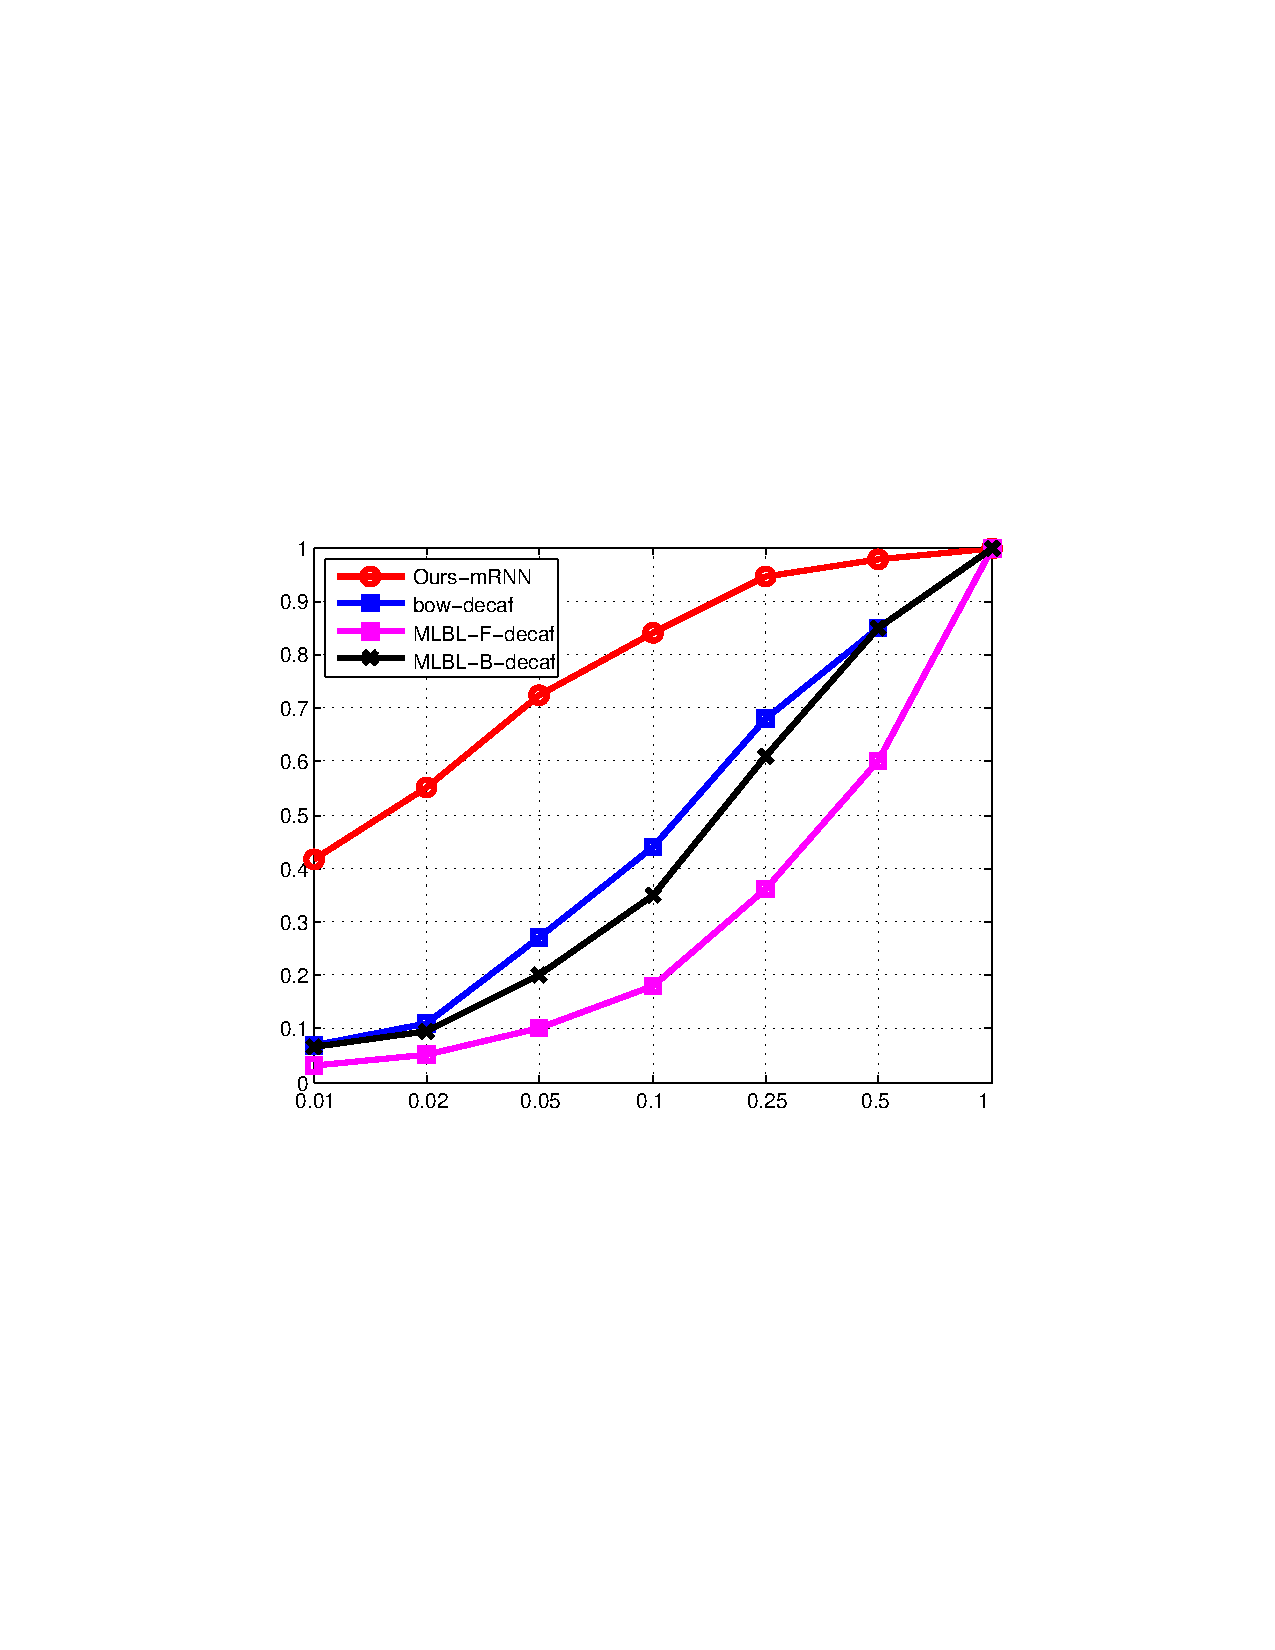
\includegraphics[width=\textwidth]{PaperFigures/I2T_iaprtc.pdf}
                \caption{Image to Text Curve}
        \end{subfigure}%
        ~ %add desired spacing between images, e. g. ~, \quad, \qquad, \hfill etc.
          %(or a blank line to force the subfigure onto a new line)
        \begin{subfigure}[b]{0.42\textwidth}
                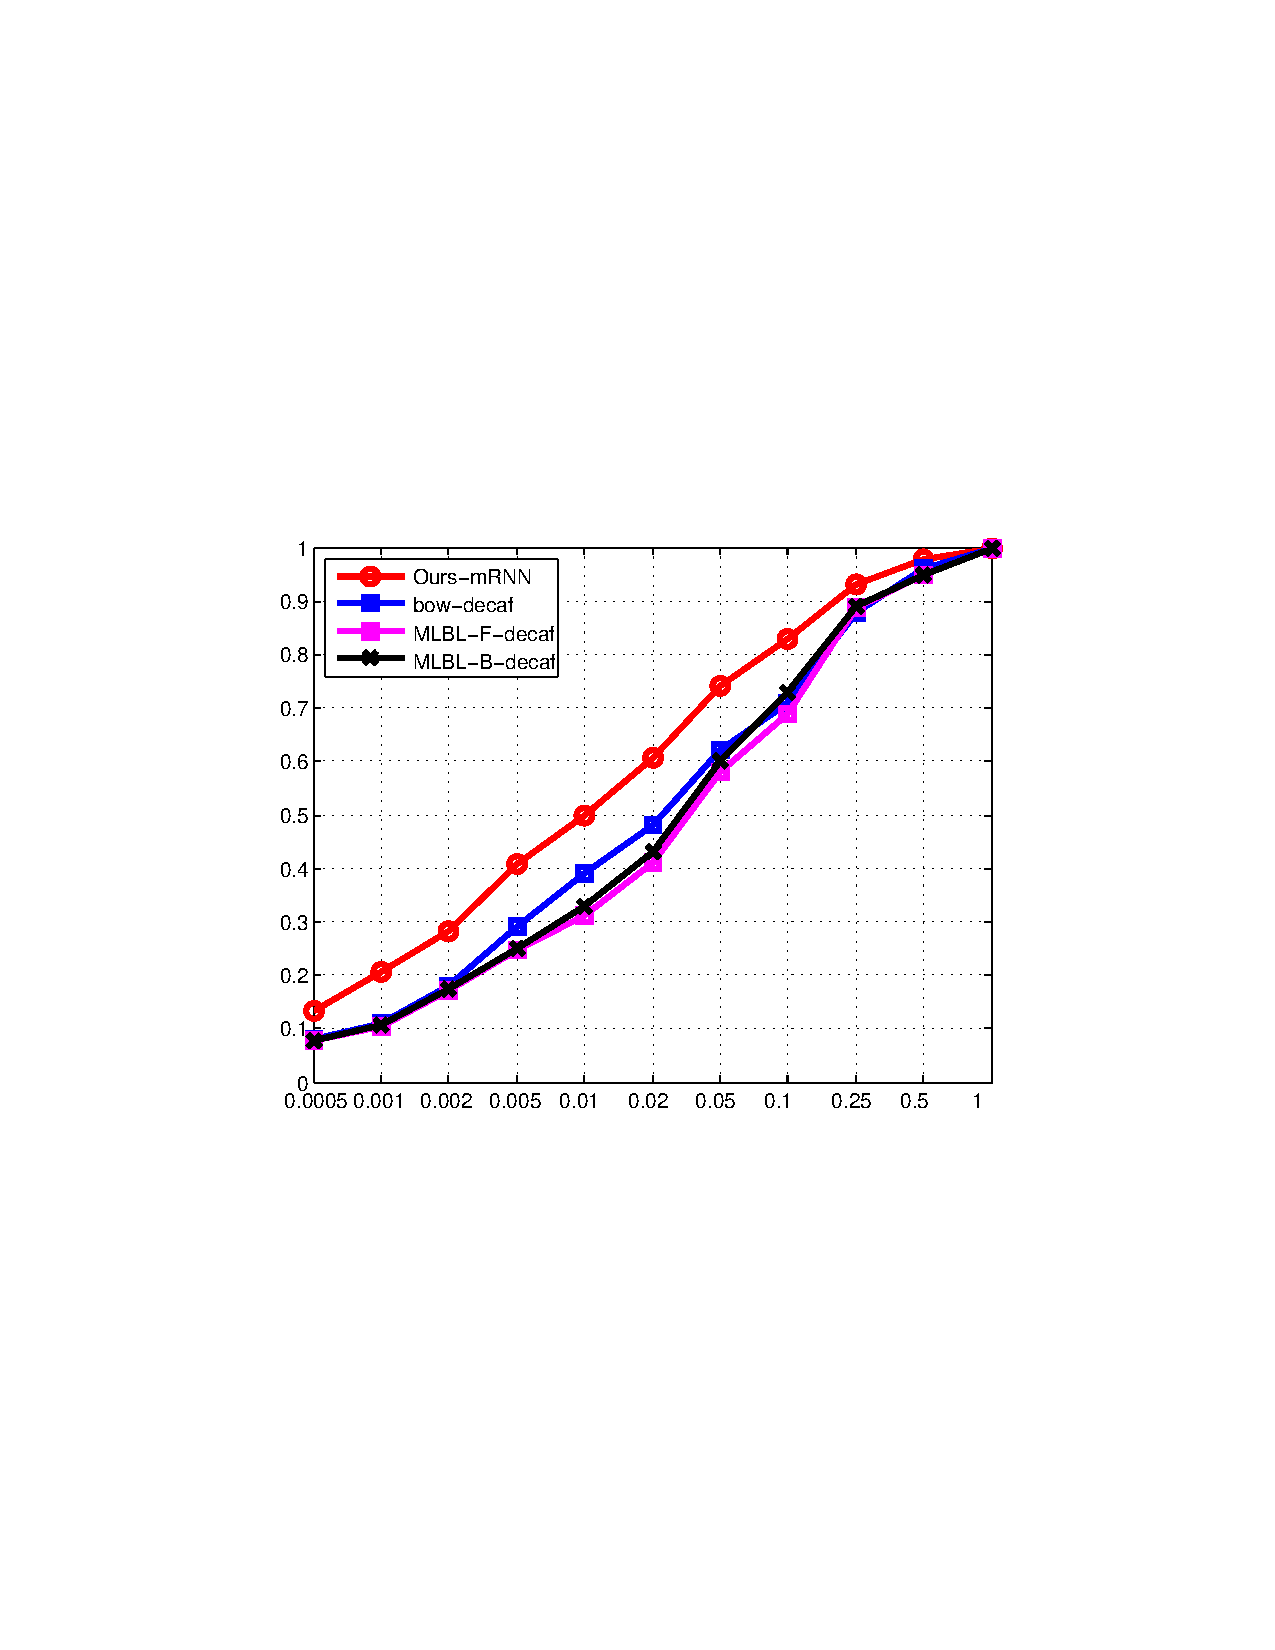
\includegraphics[width=\textwidth]{PaperFigures/T2I_iaprtc.pdf}
                \caption{Text to Image Curve}
        \end{subfigure}
        \caption{Retrieval recall curve for (a). Sentence retrieval task (Image to Text) (b). Image retrieval task (Text to Image) of iaprtc-12 dataset.}
        \label{fig:iaprtc_ret_curve}
\end{figure}

\begin{table}[htb]
	\centering
\begin{tabular}{l|cccc|cccc}
\hline
      & \multicolumn{4}{c|}{Sentence Retrival (Image to Text)} & \multicolumn{4}{c}{Image Retrival (Text to Image)} \\
\hline
      & R@1   & R@5   & R@10  & Med r & R@1   & R@5   & R@10  & Med r \\
\hline
Ours-m-RNN & 20.9  & 43.8  & 54.4  & 8     & 13.2  & 31.2  & 40.8  & 21 \\
\hline
\end{tabular}%
	\caption{Results of R@K and median rank (Med r) for iaprtc-12 dataset.}
	\label{tab:iaprtc_ret}
\end{table}

\subsection{Results on flickr8K}

This dataset was widely used for a benchmark dataset of Text to Image retrieval and Image to Text retrieval.
There are no publicly available methods that reports the statistics of generated sentences.

We first show the R@K evaluation metric in Table \ref{tab:flickr8K_ret}.
Our model outperforms the state-of-the-art methods (i.e Socher-decaf, DeViSE-decaf, DeepFE-decaf) by a large margin when using the same image features (i.e. decaf features).
In a recent work \cite{karpathy2014fragment}, they showed that using more sophisticated image features (e.g. decaf feature combined with detection results), will increase the performance.
We also list the result of the methods using such features in Talbe \ref{tab:flickr8K_ret}.
Socher-avg-rcnn and DeViSE-avg-rcnn used features of the average CNN activation of all objects above a detection confidence threshold \cite{karpathy2014fragment}.
DeepFE-rcnn used a image feature that further utilizes the RCNN detection algorithm.
Socher-avg-rcnn and DeepFE-rcnn all shows better results than their original version of Socher-decaf and DeepFE-decaf.
From the table, we can see that our method even performs better than these methods in most of the evaluation metrics.
We will develop our framework using the detection algorithm in the future work.

\begin{table}[htb]
	\centering
\begin{tabular}{l|cccc|cccc}
\hline
      & \multicolumn{4}{c|}{Sentence Retrival (Image to Text)} & \multicolumn{4}{c}{Image Retrival (Text to Image)} \\
\hline
      & R@1   & R@5   & R@10  & Med r & R@1   & R@5   & R@10  & Med r \\
\hline
Random & 0.1   & 0.5   & 1.0   & 631   & 0.1   & 0.5   & 1.0   & 500 \\
Socher-decaf \cite{socher2014grounded} & 4.5   & 18.0  & 28.6  & 32    & 6.1   & 18.5  & 29.0  & 29 \\
Socher-avg-rcnn \cite{socher2014grounded} & 6.0   & 22.7  & 34.0  & 23    & 6.6   & 21.6  & 31.7  & 25 \\
DeViSE-avg-rcnn \cite{frome2013devise} & 4.8   & 16.5  & 27.3  & 28    & 5.9   & 20.1  & 29.6  & 29 \\
DeepFE-decaf \cite{karpathy2014fragment} & 5.9   & 19.2  & 27.3  & 34    & 5.2   & 17.6  & 26.5  & 32 \\
DeepFE-rcnn \cite{karpathy2014fragment} & 12.6  & 32.9  & 44.0  & 14    & 9.7   & 29.6  & \textbf{42.5} & \textbf{15} \\
Ours-m-RNN-decaf & \textbf{14.5} & \textbf{37.2} & \textbf{48.5} & \textbf{11} & \textbf{11.5} & \textbf{31.0} & 42.4  & \textbf{15}\\
\hline
\end{tabular}%
	\caption{Results of R@K and median rank (Med r) for flickr8K dataset.}
	\label{tab:flickr8K_ret}
\end{table}

We also reports the results of generated sentences in Table \ref{tab:flickr8K_gen}.
There is no publicly available algorithm that reported results on this dataset.
We compared our m-RNN model with the Ours-RNN-Base model.
The m-RNN model performs much better than the baseline both in terms of the perplexity and BLEU scores.

\begin{table}[htb]
	\centering
\begin{tabular}{l|cccc}
\hline
      & PERP  & B-1   & B-2   & B-3 \\
\hline
Ours-RNN-Base & 30.39 & 0.4383 & 0.1849 & 0.1339 \\
Ours-m-RNN & \textbf{24.39} & \textbf{0.5778} & \textbf{0.2751} & \textbf{0.2307} \\
\hline
\end{tabular}%
	\caption{Results of generated sentences in the flickr8K dataset. }
	\label{tab:flickr8K_gen}
\end{table}

\subsection{Results on flickr30K}

This dataset is a new dataset and there are only a few methods report their retrieval results on it.
We first show the R@K evaluation metric in Table \ref{tab:flickr30K_ret}.
Our method outperforms the state-of-the-art methods in most of the evaluation metrics.

In addition, no publicly available methods reported the results of the sentence generation task as the best of our knowledge.
We report the results of generated sentences in Table \ref{tab:flickr30K_gen} with a comparison of our RNN baseline.

\begin{table}[htb]
	\centering
\begin{tabular}{l|cccc|cccc}
\hline
      & \multicolumn{4}{c|}{Sentence Retrival (Image to Text)} & \multicolumn{4}{c}{Image Retrival (Text to Image)} \\
\hline
      & R@1   & R@5   & R@10  & Med r & R@1   & R@5   & R@10  & Med r \\
Random & 0.1   & 0.6   & 1.1   & 631   & 0.1   & 0.5   & 1.0   & 500 \\
DeViSE-avg-rcnn \cite{frome2013devise} & 4.8   & 16.5  & 27.3  & 28    & 5.9   & 20.1  & 29.6  & 29 \\
DeepFE-rcnn \cite{karpathy2014fragment} & 16.4  & \textbf{40.2} & \textbf{54.7} & \textbf{8} & 10.3  & \textbf{31.4} & \textbf{44.5} & \textbf{13} \\
Ours-m-RNN-decaf & \textbf{18.4} & \textbf{40.2} & 50.9  & 10    & \textbf{12.6} & 31.2  & 41.5  & 16 \\
\hline
\end{tabular}%
	\caption{Results of R@K and median rank (Med r) for flickr30K dataset.}
	\label{tab:flickr30K_ret}
\end{table}

\begin{table}[h]
	\centering
\begin{tabular}{l|cccc}
\hline
      & PERP  & B-1   & B-2   & B-3 \\
\hline
Ours-RNN-Base & 43.96 & 0.4699 & 0.1964 & 0.1252 \\
Ours-m-RNN & \textbf{35.11} & \textbf{0.5479} & \textbf{0.2392} & \textbf{0.1952} \\
\hline
\end{tabular}%
	\caption{Results of generated sentences in the flickr8K dataset. }
	\label{tab:flickr30K_gen}
\end{table}
% To do:

\section{Conclusion}

We propose a multimodal Recurrent Neural Network framework that perform at the state-of-the-art in the tasks of sentence generation, sentence retrieval given query image and image retrieval given query sentence.
In the future work, we will try to incorporate more powerful language models and image feature extraction networks into our framework and try it on larger datasets.

{\small
\bibliographystyle{ieee}
\bibliography{egbib}
}

\end{document}
